\documentclass{article}
\usepackage{amsmath}
\usepackage{array}
\usepackage[a4paper, margin=1in]{geometry}
\usepackage{tikz}
\usetikzlibrary{decorations.pathreplacing, arrows.meta}


\begin{document}
\title{Computer System Organization - Notes}
\author{Lochana Ranatunga}
\maketitle

\section{Number Systems}
\subsection*{Decimal Number System}

We use the decimal number system in our day-to-day life.\\
Ten digits : 0,1,2,3,4,5,6,7,8,9\\
Every digit position has a weight which is a power of 10.\\
Base or radix is 10.\\

Examples:
\begin{itemize}
  \item $234 = 2 \times 10^2 + 3 \times 10^1 + 4 \times 10^0$
  \item $250.67 = 2 \times 10^2 + 5 \times 10^1 + 0 \times 10^0 + 6 \times 10^{-1} + 7 \times 10^{-2}$
\end{itemize}

\subsection*{Binary Number System}

Binary number system is used for communicating with digital devices.\\
Two digits : 0,1\\
Every digit position has a weight which is a power of 2.\\
Base or radix is 2.\\

Examples:
\begin{itemize}
  \item $110 = 1 \times 2^2 + 1 \times 2^1 + 0 \times 2^0$
  \item $101.01= 1 \times 2^2 + 0 \times 2^1 + 1 \times 2^0 + 0 \times 2^{-1} + 1 \times 2^{-2}$
\end{itemize}

\subsection*{General formula for converting any number system to decimal}
Consider a general number of base $b$ with $n$ digits and $m$ decimal points.\\
We can display the number as follows:\\
$N_b = b_{n-1}b_{n-2}...b_2b_1b_0$  .  $b_{-1}b_{-2}b_{-3}...b_{-m}$\\
\\
General formula for converting any number system to decimal:\\
$N_{b} = \sum_{i=-m}^{n-1} d_i \, b^i$\\
\\
If the integer part has $n$ digits, then highest power is: $n-1$\\
If the fractional part has m digits, then lowest power is: $-m$\\
\\
$d_i$ denotes the digit at position $i$.\\
Must satisfy: $0 \le d_i < b$\\
\\
$b$ denotes the base of the number system.\\
Like, b = 2, for binary\\
\\
Ex: Formula for Binary Numbers:\\
$B = \sum_{i=-m}^{n-1} b_i \, 2^i$\\

\subsection*{Binary to Decimal Conversion}
$101.01_2$\\

\begin{tikzpicture}[>=stealth]

% Top row
\node (a) at (0,0) {$2^2$};
\node (b) at (2,0) {$2^1$};
\node (c) at (4,0) {$2^0$};
\node (d) at (6,0) {$2^{-1}$};
\node (e) at (8,0) {$2^{-2}$};

% Bottom row (changed from -2 to -1)
\node (a2) at (0,-1) {$4$};
\node (b2) at (2,-1) {$2$};
\node (c2) at (4,-1) {$1$};
\node (d2) at (6,-1) {$\tfrac{1}{2}$};
\node (e2) at (8,-1) {$\tfrac{1}{4}$};

% Arrows
\draw[->] (a) -- (a2);
\draw[->] (b) -- (b2);
\draw[->] (c) -- (c2);
\draw[->] (d) -- (d2);
\draw[->] (e) -- (e2);

\end{tikzpicture}
\\
$101.01= 1 \times 2^2 + 0 \times 2^1 + 1 \times 2^0 + 0 \times 2^{-1} + 1 \times 2^{-2}$\\
$\phantom{00000.} =4 + 1 + 0.5 + 0.25$\\
$\phantom{00000.} = 5.75$

\subsection*{Decimal to Binary Conversion}
The reverse of binary to decimal conversion works.\\
$12 = 1 \times 2^3 + 1 \times 2^2 + 0 \times 2^1 + 0 \times 2^0$\\
\\
But, it is hard to think in reverse for large numbers.\\
Therefore, 'Successive Division' is used to convert Decimal to Binary.\\
Divide until the quotient is 0.\\
\\
Ex: (Consider remainder as R)\\
37/2 = 18 R=1\\
18/2 = 9 R=0\\
9/2 = 4 R=1\\
4/2 = 2 R=0\\
2/2 = 1 R=0\\
1/2 = 0 R=1\\\\
Now we read the remainders from bottom to top.\\
So, the converted number is, $100101_2$\\
\\When the decimal number consists of fractional parts, the fractional part and integer part are considered separately.\\
The fractional part is successively multiplied by 2, until the fractional part reaches 0.\\
Disregard integers that are created when mutliplying by 2, before the fractional part reaches 0.\\
\\
Ex:\\
$0.625 \times 2 = 1.25 \rightarrow$ here, the fractional part is 0.25 (disregard the integer part '1')\\
$0.25 \times 2 = 0.50 \rightarrow$ here, the fractional part is 0.5\\
$0.5 \times 2 = 1.00 \rightarrow$ here, the fractional part is 0\\
\\
Here, it is read from top to bottom (opposite of when the integer part is considered)\\
Therefore, the converted number is, $0.101_2$

\subsection*{Hexadecimal Number System}
Binary numbers can be displayed in a compact manner, using hexadecimal number system.\\
Group of four binary digits are represented by a hexadecimal digit.\\
Hexadecimal digits are 0 to 9, A to F.\\
\\
0 \phantom{0} 1 \phantom{0} 2 \phantom{0} 3 \phantom{0} 4 \phantom{0} 5 \phantom{0} 6 \phantom{0} 7 \phantom{0} 8 \phantom{0} 9 \phantom{0} 10 \phantom{0} 11 \phantom{0} 12 \phantom{0} 13 \phantom{0} 14 \phantom{0} 15\\
0 \phantom{0} 1 \phantom{0} 2 \phantom{0} 3 \phantom{0} 4 \phantom{0} 5 \phantom{0} 6 \phantom{0} 7 \phantom{0} 8 \phantom{0} 9 \phantom{0} A \phantom{00} B \phantom{00} C \phantom{0} D \phantom{00} E \phantom{00} F\\
\\
Ways to display hexadecimal numbers:\\
Prefixing 0x or suffixing H.\\
\\
Ex:\\
$2AH = 0x2A$
\newpage
\subsection*{Binary to Hexadecimal Conversion}
Pair digits by 4, from Right to Left in the integer side, and from Left to Right in the fractional part.\\
\\
\\
\begin{tikzpicture}[>=Stealth]

% Bit strings
\node at (0,0)  {1101};
\node at (3,0)  {1110};
\node at (4.5,0) {.};
\node at (6,0)  {0010};
\node at (8.5,0){1100};

% Braces and labels
\draw[decorate,decoration={brace,mirror,amplitude=6pt}]
(-0.8,-0.3) -- (0.8,-0.3) node[midway,yshift=-0.6cm]{13};

\draw[decorate,decoration={brace,mirror,amplitude=6pt}]
(2.2,-0.3) -- (3.8,-0.3) node[midway,yshift=-0.6cm]{14};

\draw[decorate,decoration={brace,mirror,amplitude=6pt}]
(5.2,-0.3) -- (6.8,-0.3) node[midway,yshift=-0.6cm]{2};

\draw[decorate,decoration={brace,mirror,amplitude=6pt}]
(7.7,-0.3) -- (9.3,-0.3) node[midway,yshift=-0.6cm]{12};

% Down arrows and labels
\draw[->] (0,-1.2) -- (0,-2) node[below]{D};
\draw[->] (3,-1.2) -- (3,-2) node[below]{E};
\draw[->] (8.5,-1.2) -- (8.5,-2) node[below]{C};

% Left arrow (shifted slightly right)
\draw[<-] (-1.0,1) -- (3.8,1);

% Right arrow (unchanged or slightly adjusted)
\draw[->] (5.0,1) -- (9.5,1);

\end{tikzpicture}
\\
\\
So, $11011110_2 = DE.2C_{16}$
\subsection*{Hexadecimal to Binary Conversion}

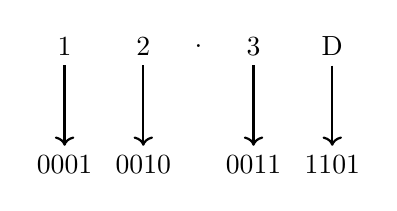
\begin{tikzpicture}[node distance=1.5cm]
    % Place the Hexadecimal/Decimal characters
    \node (H1) {1};
    \node (H2) [right of=H1, xshift=-0.5cm] {2};
    \node (DOT) [right of=H2, xshift=-0.8cm] {$.$};
    \node (H3) [right of=DOT, xshift=-0.8cm] {3};
    \node (H4) [right of=H3, xshift=-0.5cm] {D};

    % Place the Binary groups below
    \node (B1) [below of=H1] {0001};
    \node (B2) [below of=H2] {0010};
    \node (B3) [below of=H3] {0011};
    \node (B4) [below of=H4] {1101};

    % Draw the arrows
    \draw[->, thick] (H1) -- (B1);
    \draw[->, thick] (H2) -- (B2);
    \draw[->, thick] (H3) -- (B3);
    \draw[->, thick] (H4) -- (B4);
\end{tikzpicture}\\
\\
So, $12.3D_{16} = 10010.00111101_2$
\subsection*{Unsigned Binary Numbers}
Unsigned binary numbers are, binary numbers without a sign.\\
Or else, positive integers.\\
Unsigned binary numbers can be displayed as usual, using standard decimal to binary conversion.\\
Range: $ 0 \rightarrow  2^n - 1$
\subsection*{Signed Binary Numbers}
Signed binary numbers have a sign.\\
Therefore, 1 bit is used to display the sign, and the rest are used to display the number.\\
There are a few ways we can represent signed binary numbers.
\subsubsection*{a - Sign Magnitude Representation}
Here, the most significant bit (MSB) is used to display the sign.\\
The most significant bit is the bit with the largest power of 2 weight from the sequence.\\
When MSB = 0, the sign is "Positive", while when MSB = 1,  the sign is "Negative".\\
\\
Ex:\\
0011 = +3\\
1011 = -3\\
\\
A disadvantage of this method is, that 0, can be displayed in 2 ways. (+0/-0)\\
Range: $-(2^{n-1} - 1) \rightarrow +(2^{n-1} - 1)$
\newpage
\subsubsection*{b - One's Complement Representation}
Here, we display positive numbers using the previous "Sign Magnitude Representation" method, and flip the digits to make it negative.\\
\\
Ex:\\
$0001_2 = +1 \rightarrow 1110_2 = -1$\\
$0101_2 = +5 \rightarrow 1010_2 = -5$\\
\\
Also here, a disadvantage is, that 0, can be displayed in 2 ways. (-0/+0)\\
Range: $-(2^{n-1} - 1) \rightarrow +(2^{n-1} - 1)$

\end{document}